\section{Durchführung}
\label{sec:Durchführung}
Um sowohl die Strahlen- als auch die Wellenoptik genauer zu untersuchen,wird
eine Grundplatte verwendet, unter der unterschiedliche Vorlagen mit Winkelskalen
platziert werden können. Darauf befestigt sind zwei Laserdioden, eine mit der 
Wellenlänge $\lambda_r = 635 \si{\nano\m}$, also rotem Licht, und eine mit
Wellenlänge $\lambda_g = 532 \si{\nano\m}$, grünem Licht, die im 
Halbkreis bewegt werden können.\\
Des weiteren werden für die unterschiedlichen Versuche verschiedene optische
Elemente (zu sehen in Abbildung \ref{fig:elemente}) im Zentrum des Halbkreises platziert.

\begin{figure}
    \centering
    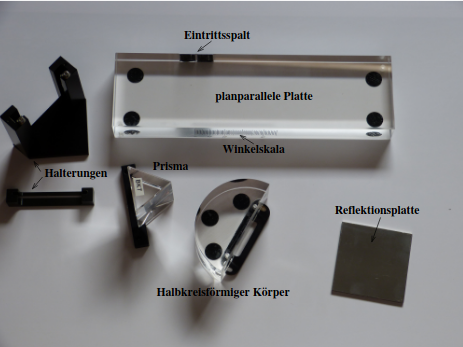
\includegraphics[width=0.75\textwidth]{werkzeug.png}
    \caption{Optische Elemente für verschiedene Untersuchungen. (Quelle \cite{versuch})}
    \label{fig:elemente}
\end{figure}

\subsection{Reflexion}
Zunächst wird ein Spiegel im Zentrum des Halbkreises platziert. Der Versuchsaufbau
ist in Abbildung \ref{fig:aufbau} gezeigt.

\begin{figure}
    \centering
    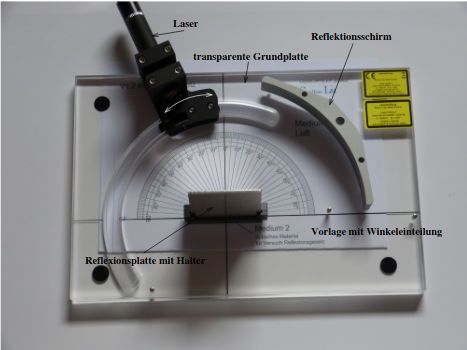
\includegraphics[width=0.75\textwidth]{aufbauuu.png}
    \caption{Versuchsaufbau zur Untersuchung der Reflexion. (Quelle \cite{versuch})}
    \label{fig:aufbau}
\end{figure}

Mit dem grünen Laser wird für 7 Einfallswinkel der Reflexionswinkel gemessen.

\subsection{Brechung}
Um die Brechung im optisch dichteren Medium zu betrachten, wird eine Plexiglasplatte
mit einer an einer Seite angeklebten Winkelskala,
wie sie in Abbildung \ref{fig:elemente} zu sehen ist, verwendet. Die 
Platte wird so platziert, dass der Eintrittsspalt zur Winkelskala zeigt.
Auch hier werden 7 Einfallswinkel betrachtet.

\subsection{Planparallele Platten}
Der Versuch wird analog wie der zur Brechung aufgebaut. Zusätzlich wird
ein Transmissionsschirm aufgestellt. Mit dem grünen Laser wird
für 5 Einfallswinkel der Strahlversatz gemessen.

\subsection{Prisma}
Zur Betrachtung der Brechung am Prisma wird im Zentrum des Halbkreises
ein Prisma aus Kronglas platziert. Um die Dispersion zu messen, wird
für den roten Laser bei 5 Einfallswinkeln die Ablenkung gemessen.

\subsection{Beugung am Gitter}
Zunächst wird der Versuch ohne Beugungsgitter in der Mitte des Halbkreises aufgebaut.
Dabei trifft das Laserlicht den Transmissionsschirm bei einem Winkel von 0 Grad. 
Es werden für drei Beugungsgitter unterschiedlicher Gitterkonstante mit dem roten Laser die 
Maxima gemessen. 